% =============================================================================
% SECCIÓN 2.5: LÓGICA DIFUSA Y SISTEMAS DE INFERENCIA MAMDANI
% =============================================================================

\section{Lógica Difusa y Sistemas de Inferencia Mamdani}
\label{sec:logica_difusa}

La lógica difusa y los sistemas de inferencia Mamdani proporcionan un marco formal para modelar razonamiento humano impreciso mediante variables lingüísticas, conjuntos difusos y reglas del tipo ``SI-ENTONCES'', y se han aplicado extensamente a la clasificación de estados de congestión vehicular en sistemas de transporte inteligente (ITS). Esta sección resume los fundamentos matemáticos de la lógica difusa, las funciones de membresía más utilizadas, la arquitectura del sistema Mamdani y ejemplos representativos de su uso en clasificación de tráfico.

\subsubsection{Fundamentos de Lógica Difusa}

La lógica difusa surge como una generalización de la lógica clásica binaria para tratar conceptos vagos como ``bajo'', ``medio'' o ``alto'', donde la pertenencia de un elemento a una clase no es dicotómica sino gradual. Zadeh define un conjunto difuso $\tilde{A}$ sobre un universo $X$ mediante una función de membresía $\mu_{\tilde{A}}: X \rightarrow [0,1]$, donde $\mu_{\tilde{A}}(x)$ indica el grado de pertenencia de $x$ al conjunto \cite{zadeh1965fuzzy}. Esta formalización permite extender nociones clásicas como unión, intersección y complemento a un contexto continuo, manteniendo propiedades de convexidad y posibilitando teoremas de separación para conjuntos difusos.

En lógica difusa, una variable lingüística es una variable cuyo valor son términos lingüísticos (por ejemplo, ``velocidad'' con valores $\{$muy baja, baja, media, alta, muy alta$\}$), y cada término se representa como un conjunto difuso sobre el dominio numérico correspondiente. Una proposición difusa, como ``la velocidad es alta'', se interpreta como un grado en $[0,1]$ obtenido evaluando la función de membresía asociada al término ``alta'' en el valor numérico observado de la velocidad \cite{zadeh1971similarity}. Esta capacidad de modelar gradualidad es fundamental en aplicaciones donde los conceptos no tienen límites precisos, como en la clasificación de estados de tráfico donde la transición entre ``flujo libre'' y ``congestión'' es continua y subjetiva.

\subsubsection{Funciones de Membresía}

Las funciones de membresía definen la forma de los conjuntos difusos e influyen directamente en la suavidad del razonamiento y en la sensibilidad del sistema. En aplicaciones de control e ITS se utilizan habitualmente funciones de tipo triangular, trapezoidal y gaussiana, debido a su simplicidad y a la facilidad de parametrización.

La función de membresía triangular está definida por tres parámetros $(a, b, c)$ que determinan el inicio, el pico y el final del soporte, y su expresión típica es:

\begin{equation}
\mu(x) = 
\begin{cases}
0, & x \le a \\
\frac{x-a}{b-a}, & a < x \le b \\
\frac{c-x}{c-b}, & b < x < c \\
0, & x \ge c
\end{cases}
\end{equation}

Esta función proporciona una transición lineal suave con máximo igual a 1 en $b$ y se usa extensamente cuando se requiere una implementación computacional ligera, como en sistemas embebidos para control de tráfico en tiempo real.

La función trapezoidal generaliza la triangular añadiendo una meseta central, y se define por cuatro parámetros $(a, b, c, d)$ con:

\begin{equation}
\mu(x) =
\begin{cases}
0, & x \le a \\
\frac{x-a}{b-a}, & a < x \le b \\
1, & b < x \le c \\
\frac{d-x}{d-c}, & c < x < d \\
0, & x \ge d
\end{cases}
\end{equation}

Esta función permite modelar rangos donde el grado de pertenencia se considera plenamente verdadero en un intervalo y se degrada linealmente en los extremos. Cuando $b = c$, la trapezoidal se reduce a una triangular, proporcionando flexibilidad en el modelado de conceptos que tienen una zona central de certeza máxima.

La función de membresía gaussiana se caracteriza por parámetros $c$ (centro) y $\sigma$ (desviación estándar):

\begin{equation}
\mu(x) = \exp\left( -\frac{(x-c)^2}{2\sigma^2} \right)
\end{equation}

Esta función produce una transición suave e infinitamente diferenciable, lo que resulta útil cuando se desean gradientes suaves o se combinan sistemas difusos con métodos de optimización continua. En sistemas de clasificación y control adaptativo, las gaussianas suelen proporcionar un ajuste más realista de distribuciones empíricas a costa de mayor complejidad de parametrización.

La Figura~\ref{fig:fuzzy_velocidad} ilustra cómo una variable numérica (velocidad promedio) se mapea a términos lingüísticos mediante funciones de membresía de diferentes tipos, mostrando la superposición de conjuntos difusos y cómo un valor crisp genera múltiples grados de pertenencia simultáneos.

\begin{figure}[htbp]
\centering
\shorthandoff{>}
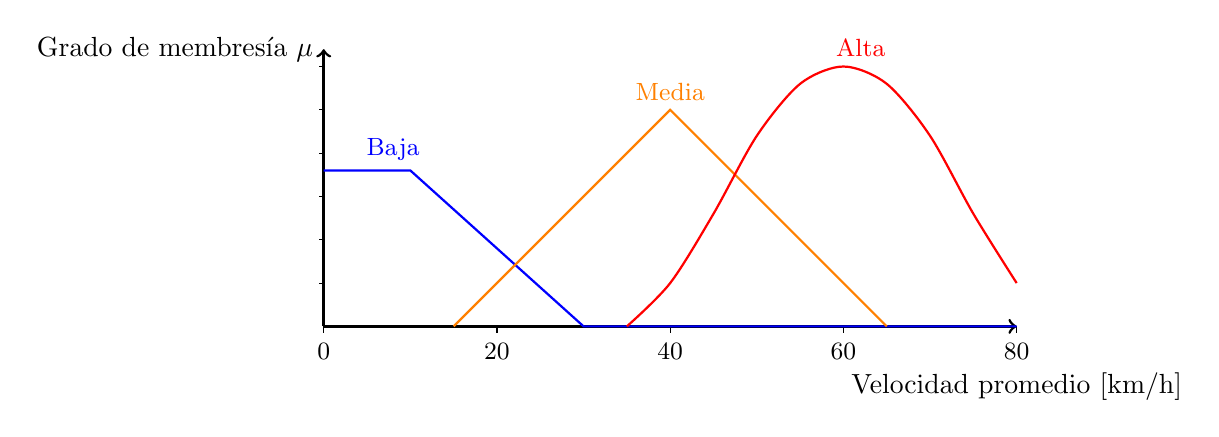
\begin{tikzpicture}[scale=1.1]
    % Ejes
    \draw[->,line width=1pt] (0,0) -- (8,0) node[below,yshift=-0.45cm] {Velocidad promedio [km/h]};
    \draw[->,line width=1pt] (0,0) -- (0,3.2) node[left] {Grado de membres\'ia $\mu$};

    % Marcas en eje x
    \foreach \x/\label in {0/0,2/20,4/40,6/60,8/80} {
        \draw (\x,0) -- (\x,-0.08) node[below] {\small \label};
    }

    % Baja: trapezoidal
    \draw[thick,blue]
        (0,1.8) -- (1,1.8) -- (3,0) -- (8,0);
    \node[blue,above] at (0.8,1.8) {\small Baja};

    % Media: triangular
    \draw[thick,orange]
        (1.5,0) -- (4,2.5) -- (6.5,0);
    \node[orange,above] at (4,2.5) {\small Media};

    % Alta: gaussiana aproximada
    \draw[thick,red,smooth] plot coordinates
        {(3.5,0) (4.0,0.5) (4.5,1.3) (5.0,2.2) (5.5,2.8) (6.0,3.0)
         (6.5,2.8) (7.0,2.2) (7.5,1.3) (8.0,0.5)};
    \node[red,above] at (6.2,3.0) {\small Alta};

    % Eje y marcas
    \foreach \y in {0.5,1,1.5,2,2.5,3} {
        \draw (0,\y) -- (-0.06,\y);
    }
\end{tikzpicture}
\shorthandon{>}
\caption{Variable ling\"u\'istica \emph{velocidad promedio} con tres conjuntos difusos (baja, media, alta) modelados mediante funciones de membres\'ia trapezoidal, triangular y aproximadamente gaussiana.}
\label{fig:fuzzy_velocidad}
\end{figure}

\subsubsection{Sistema de Inferencia Mamdani}

El sistema de inferencia Mamdani fue introducido por Mamdani y Assilian como un enfoque para implementar controladores basados en reglas lingüísticas expresadas por expertos humanos \cite{mamdani1975experiment}. Este tipo de sistema se caracteriza porque tanto los antecedentes como los consecuentes de las reglas son conjuntos difusos y porque la salida final se obtiene mediante un proceso de defuzzificación de un conjunto difuso agregado.

Un sistema Mamdani típico consta de cuatro etapas principales. La primera etapa es la fuzzificación, donde los valores de entrada crisp (numéricos) se transforman en grados de pertenencia a los conjuntos difusos definidos para cada variable lingüística de entrada. Para cada valor de entrada $x_i$ y cada término lingüístico $A_{ij}$, se calcula $\mu_{A_{ij}}(x_i)$, generando un vector de pertenencias que alimenta el motor de inferencia.

La segunda etapa es la evaluación de reglas (inferencia local). Las reglas Mamdani suelen tener la forma:

\begin{equation}
\text{SI } x_1 \text{ es } A_{k1} \text{ Y } x_2 \text{ es } A_{k2} \text{ ENTONCES } y \text{ es } B_k
\end{equation}

Los antecedentes se combinan mediante operadores t-norma (típicamente mínimo o producto) y t-conorma (máximo para OR) para obtener el grado de activación de cada regla. Este grado escala el conjunto difuso consecuente $B_k$, generando una salida difusa por regla mediante implicación min o producto.

La tercera etapa es la agregación de salidas. Las salidas difusas de todas las reglas se combinan en un único conjunto difuso de salida usando generalmente el operador máximo punto a punto sobre el universo de discurso de la variable de salida. El resultado es la salida agregada, que representa la contribución conjunta de todas las reglas del sistema para el vector de entrada dado.

La cuarta etapa es la defuzzificación. La salida agregada es un conjunto difuso que debe convertirse en un valor numérico (crisp) para su uso en control o decisión. El método de defuzzificación más empleado en sistemas Mamdani es el centroide o centro de gravedad (COG), calculado como:

\begin{equation}
y^* = \frac{\int y \, \mu_{\text{out}}(y) \, dy}{\int \mu_{\text{out}}(y) \, dy}
\end{equation}

donde $\mu_{\text{out}}$ es la función de membresía del conjunto de salida agregado. Otros métodos incluyen el máximo de la media (mean of maxima) o el máximo del máximo (argmax), pero el centroide suele ofrecer un compromiso adecuado entre estabilidad y sensibilidad.

El trabajo original de Mamdani demostró que un controlador difuso basado en reglas lingüísticas podía igualar o superar el desempeño de controladores clásicos para una planta de vapor, estableciendo la viabilidad práctica de este enfoque \cite{mamdani1975experiment}.

La Figura~\ref{fig:mamdani_flujo} muestra el flujo completo de un sistema Mamdani, desde las entradas numéricas hasta la salida crisp, ilustrando las cuatro etapas principales del proceso de inferencia.

\begin{figure}[htbp]
\centering
\shorthandoff{>}
\begin{tikzpicture}[node distance=1.4cm,>=latex]

    \tikzstyle{block} = [rectangle, draw, rounded corners,
                         text width=5cm, align=center,
                         minimum height=0.9cm, font=\small]
    \tikzstyle{line} = [draw,->]

    % Nodos organizados verticalmente
    \node[block] (inputs) {Entradas \emph{crisp}:\\
        velocidad promedio, densidad, flujo};
    \node[block, below=of inputs] (fuzz) {Fuzzificaci\'on:\\
        asignaci\'on de grados de pertenencia a conjuntos difusos (bajo/medio/alto)};
    \node[block, below=of fuzz] (rules) {Base de reglas Mamdani:\\
        SI velocidad es alta Y densidad es alta ENTONCES congesti\'on es severa, ...};
    \node[block, below=of rules] (agg) {Inferencia y agregaci\'on:\\
        combinaci\'on de salidas de reglas (t-norma, t-conorma, m\'aximo)};
    \node[block, below=of agg] (defuzz) {Defuzzificaci\'on:\\
        c\'alculo del centroide $\rightarrow$ nivel de congesti\'on \emph{crisp}};
    \node[block, below=of defuzz] (output) {Salida \emph{crisp}:\\
        nivel de congesti\'on / decisi\'on de control};

    % Flechas verticales con etiquetas a la derecha
    \path[line] (inputs) -- node[right,font=\small]{valores medidos} (fuzz);
    \path[line] (fuzz) -- node[right,font=\small]{grados de pertenencia} (rules);
    \path[line] (rules) -- node[right,font=\small]{salidas difusas por regla} (agg);
    \path[line] (agg) -- node[right,font=\small]{conjunto difuso agregado} (defuzz);
    \path[line] (defuzz) -- node[right,font=\small]{valor \emph{crisp}} (output);

\end{tikzpicture}
\shorthandon{>}
\caption{Flujo de un sistema de inferencia difusa tipo Mamdani: de entradas num\'ericas a una salida \emph{crisp} mediante fuzzificaci\'on, reglas, agregaci\'on y defuzzificaci\'on.}
\label{fig:mamdani_flujo}
\end{figure}

La Figura~\ref{fig:regla_mamdani} ilustra el funcionamiento de una regla individual, mostrando cómo los grados de pertenencia de las entradas se combinan para activar el consecuente difuso con un grado de activación determinado.

\begin{figure}[htbp]
    \centering
    \shorthandoff{>}
    \begin{tikzpicture}[>=latex,scale=1.0]
    
    % =========================
    % ENTRADAS — FUZZIFICACIÓN
    % =========================
    
    \begin{scope}[shift={(0,0)}]
        \node[font=\bfseries\normalsize] at (1.8,3.6) {Fuzzificación};
    
        % Velocidad
        \draw[->] (0,0) -- (3.4,0) node[below] {Velocidad};
        \draw[->] (0,0) -- (0,2.2) node[left] {$\mu$};
    
        \draw[thick,blue] (0.3,0) -- (1.4,2.0) -- (3.0,0);
        \node[blue,above] at (1.4,2.0) {\small Alta};
    
        \draw[dashed] (2.2,0) -- (2.2,1.2);
        \fill (2.2,1.2) circle (1.6pt);
        \draw[dashed] (0,1.2) -- (2.2,1.2);
        \node[left,font=\small] at (0,1.2) {$\mu_{\text{vel}}$};
    
        \coordinate (velAct) at (2.2,1.2);
    \end{scope}
    
    \begin{scope}[shift={(0,-3.4)}]
        % Densidad
        \draw[->] (0,0) -- (3.4,0) node[below] {Densidad};
        \draw[->] (0,0) -- (0,2.2) node[left] {$\mu$};
    
        \draw[thick,orange] (0.3,0) -- (1.6,2.0) -- (3.0,0);
        \node[orange,above] at (1.6,2.0) {\small Alta};
    
        \draw[dashed] (1.9,0) -- (1.9,1.5);
        \fill (1.9,1.5) circle (1.6pt);
        \draw[dashed] (0,1.5) -- (1.9,1.5);
        \node[left,font=\small] at (0,1.5) {$\mu_{\text{dens}}$};
    
        \coordinate (densAct) at (1.9,1.5);
    \end{scope}
    
    % =========================
    % REGLA
    % =========================
    
    \node[
        draw,
        rounded corners,
        fill=gray!8,
        align=center,
        font=\small,
        text width=3.6cm
    ] (rule) at (6.6,-1.7)
    {
    \textbf{Regla $R_k$}\\[0.4em]
    $\begin{aligned}
    \text{vel} &= \text{alta}\\
    \text{dens} &= \text{alta}
    \end{aligned}$\\[0.4em]
    $\Rightarrow$ cong = severa\\[0.6em]
    $\alpha_k = \min(\mu_{\text{vel}},\mu_{\text{dens}})$
    };
    
    % Flechas entradas → regla (más aire)
    \draw[->] (velAct) -- (rule.west |- 6.6,-0.8);
    \draw[->] (densAct) -- (rule.west |- 6.6,-2.6);
    
    % =========================
    % SALIDA — IMPLICACIÓN
    % =========================
    
    \begin{scope}[shift={(11.0,-1.7)}]
        \node[font=\bfseries\normalsize] at (1.9,3.6) {Implicación};
    
        \draw[->] (0,0) -- (3.6,0) node[below] {Congestión};
        \draw[->] (0,0) -- (0,2.5) node[left] {$\mu$};
    
        \draw[thick,red] (1.0,0) -- (2.2,2.0) -- (3.4,2.0);
        \node[red,above] at (2.4,2.0) {\small Severa};
    
        \draw[dashed] (0,1.0) -- (3.6,1.0);
        \node[left,font=\small] at (0,1.0) {$\alpha_k$};
    
        \clip (0,0) rectangle (3.6,1.0);
        \draw[thick,red,fill=red!20] (1.0,0) -- (2.2,2.0) -- (3.4,2.0);
    
        \coordinate (outWest) at (0,1.2);
    \end{scope}
    
    % Flecha regla → salida (aire y etiqueta envuelta)
    \draw[->,thick] (rule.east) -- (outWest)
        node[midway,above,align=center,font=\small]
        {Implicación\\Mamdani};
    
    \end{tikzpicture}
    \shorthandon{>}
    \caption{Inferencia difusa tipo Mamdani para una regla individual. Las entradas se fuzzifican, se combinan mediante un operador Y y activan el consecuente mediante recorte con grado $\alpha_k$.}
    \label{fig:regla_mamdani}
    \end{figure}
    
    

\subsubsection{Aplicación en Clasificación de Congestión Vehicular}

En sistemas de transporte inteligente, la lógica difusa se utiliza ampliamente para modelar la percepción humana de la congestión y para construir clasificadores que estimen el estado del tráfico a partir de variables macroscópicas como flujo, velocidad y densidad. La naturaleza gradual de conceptos como ``flujo alto'' o ``velocidad baja'' se adapta de forma natural al formalismo de variables lingüísticas y conjuntos difusos, evitando umbrales rígidos que pueden ser sensibles al ruido.

La Figura~\ref{fig:fuzzy_congestion_its} muestra un ejemplo de integración de un sistema difuso Mamdani en un entorno ITS, ilustrando el flujo desde la captura de datos de sensores hasta la generación de recomendaciones para el control de tráfico.

Un esquema típico de clasificación difusa de congestión vehicular con sistema Mamdani incluye la selección de variables de entrada. Variables macroscópicas como flujo (vehículos/hora), velocidad media (km/h) y densidad (vehículos/km) son comúnmente utilizadas. Algunos trabajos consideran adicionalmente ocupación o tiempo de viaje para capturar mejor la variabilidad del tráfico.

El diseño de variables lingüísticas y funciones de membresía implica que cada variable se discretiza en términos lingüísticos como ``bajo'', ``medio'', ``alto'', ``muy alto'', representados con funciones de membresía triangulares o trapezoidales sobre rangos calibrados a partir de datos empíricos. La calibración suele hacerse con apoyo de expertos en tráfico o mediante técnicas de clustering como fuzzy c-means para determinar automáticamente los puntos de corte.

La definición de reglas Mamdani construye una base de reglas del tipo: ``SI flujo es bajo Y velocidad es alta ENTONCES congestión es libre'', o ``SI flujo es alto Y velocidad es baja Y densidad es alta ENTONCES congestión es severa''. Estas reglas reflejan conocimiento experto o patrones encontrados en los datos históricos, permitiendo capturar relaciones no lineales entre variables de tráfico que serían difíciles de modelar con técnicas deterministas.

El proceso de inferencia y clasificación de estado permite que el sistema Mamdani procese en tiempo (casi) real las mediciones procedentes de detectores o sensores y devuelva un nivel de congestión difuso que se defuzzifica a categorías discretas como $\{$libre, estable, inestable, congestionado$\}$. Estudios recientes muestran que estos clasificadores difusos son robustos ante datos incompletos o ruidosos y capturan de manera más fiel la percepción de los conductores respecto a soluciones crisp basadas en umbrales fijos \cite{musriroh2020application, esmaeili2025optimization}.

En el contexto de sistemas de gestión de tráfico urbano, los sistemas de inferencia difusa tipo Mamdani permiten transformar variables como velocidad promedio, densidad vehicular y flujo en categorías lingüísticas (``bajo'', ``medio'', ``alto'') mediante funciones de membresía, y combinar reglas del tipo ``si-entonces'' para clasificar el grado de congestión en niveles como ``leve'', ``moderada'' o ``severa'', facilitando la toma de decisiones bajo incertidumbre inherente a la variabilidad del tráfico urbano.

\begin{figure}[htbp]
\centering
\shorthandoff{>}
\begin{tikzpicture}[node distance=1.4cm,>=latex]

    \tikzstyle{block} = [rectangle, draw, rounded corners,
                         text width=5cm, align=center,
                         minimum height=0.9cm, font=\small]

    % Bloques organizados verticalmente
    \node[block] (sensors) {Intersecci\'on urbana con sensores:\\
        bucles inductivos, c\'amaras, contadores};

    % Medición
    \node[block, below=of sensors] (measure) {Medici\'on de variables};

    % Sistema Mamdani
    \node[block, below=of measure] (mamdani) {Sistema de inferencia difusa Mamdani:\\
        fuzzificaci\'on + reglas + agregaci\'on + defuzzificaci\'on};

    % Módulo de decisión
    \node[block, below=of mamdani] (decision) {M\'odulo de decisi\'on / control:\\
        ajuste de tiempos semaf\'oricos u otras acciones};

    % Flechas verticales con etiquetas a la derecha
    \draw[->] (sensors) -- node[right,font=\small]{datos de tr\'afico} (measure);
    \draw[->] (measure) -- node[right,font=\small]{entradas \emph{crisp}} (mamdani);
    \draw[->] (mamdani) -- node[right,font=\small]{nivel de congesti\'on} (decision);

\end{tikzpicture}
\shorthandon{>}
\caption{Ejemplo de integraci\'on de un sistema difuso Mamdani en un entorno ITS para clasificar congesti\'on y alimentar un m\'odulo de decisi\'on o control semaf\'orico.}
\label{fig:fuzzy_congestion_its}
\end{figure}

La aplicación de lógica difusa Mamdani al control de semáforos y a la gestión dinámica de tráfico ha sido ampliamente documentada en la literatura. Diversos estudios reportan mejoras en tiempos de viaje y reducción en el número de paradas frente a esquemas de control fijo \cite{musriroh2020application, esmaeili2025optimization, erdinc2023application}. Por ejemplo, Erdinç propone un identificador difuso de estado de tráfico basado en Mamdani que utiliza flujo, velocidad y densidad como entradas y produce una clasificación continua del estado de congestión, demostrando que el modelo captura correctamente las transiciones entre flujo libre y condiciones hipercríticas \cite{erdinc2023application}. Otros trabajos aplican lógica difusa Mamdani al control de semáforos y a la gestión dinámica de carriles, mostrando reducciones significativas en tiempos de viaje y número de paradas frente a esquemas de control fijo \cite{musriroh2020application, esmaeili2025optimization}. Estas evidencias posicionan a la lógica difusa Mamdani como una herramienta valiosa en sistemas de optimización de tráfico urbano que requieren adaptabilidad y robustez ante condiciones variables.

